\section{Ordenacao e ordenação invertida}
Todos os algoritmos e suas variações estão implementados no codigo a seguir. 

Para testramos a funcionalidade dos algoritmos utilizamos um argumento na main para escolher uma das possibilidades de algoritmos. 

Parâmetros: 
\begin{itemize}
	\item 1 -- Shellsort
	\item 12 -- Shellsort Reverso
	\item 2 -- Quicksort 
	\item 22 -- Quicksort Reverso
	\item 3 -- Heapsort
	\item 32 -- Heapsort Reverso
	\item 4 -- Mergesort
	\item 42 -- Mergesort Reverso
\end{itemize}

Resultados: 
Printamos as primeiras $30$ posições do vetor após a ordenação

\begin{figure}[h!]
	\centering

	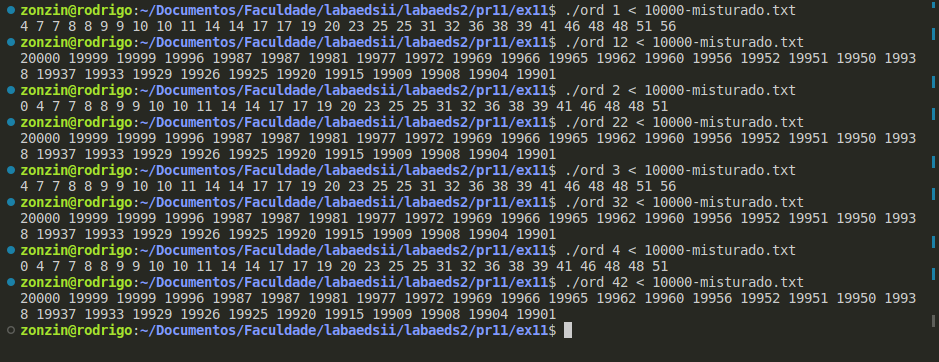
\includegraphics[width=10cm]{imgs/resultadoAlgoritmos.png}

	\caption{Todos os algoritmos}
\end{figure}

\newpage
\section{Tempos}
Usando o script em Python, obtemos os seguintes tempos: 

\begin{figure}[h!]
	\centering
	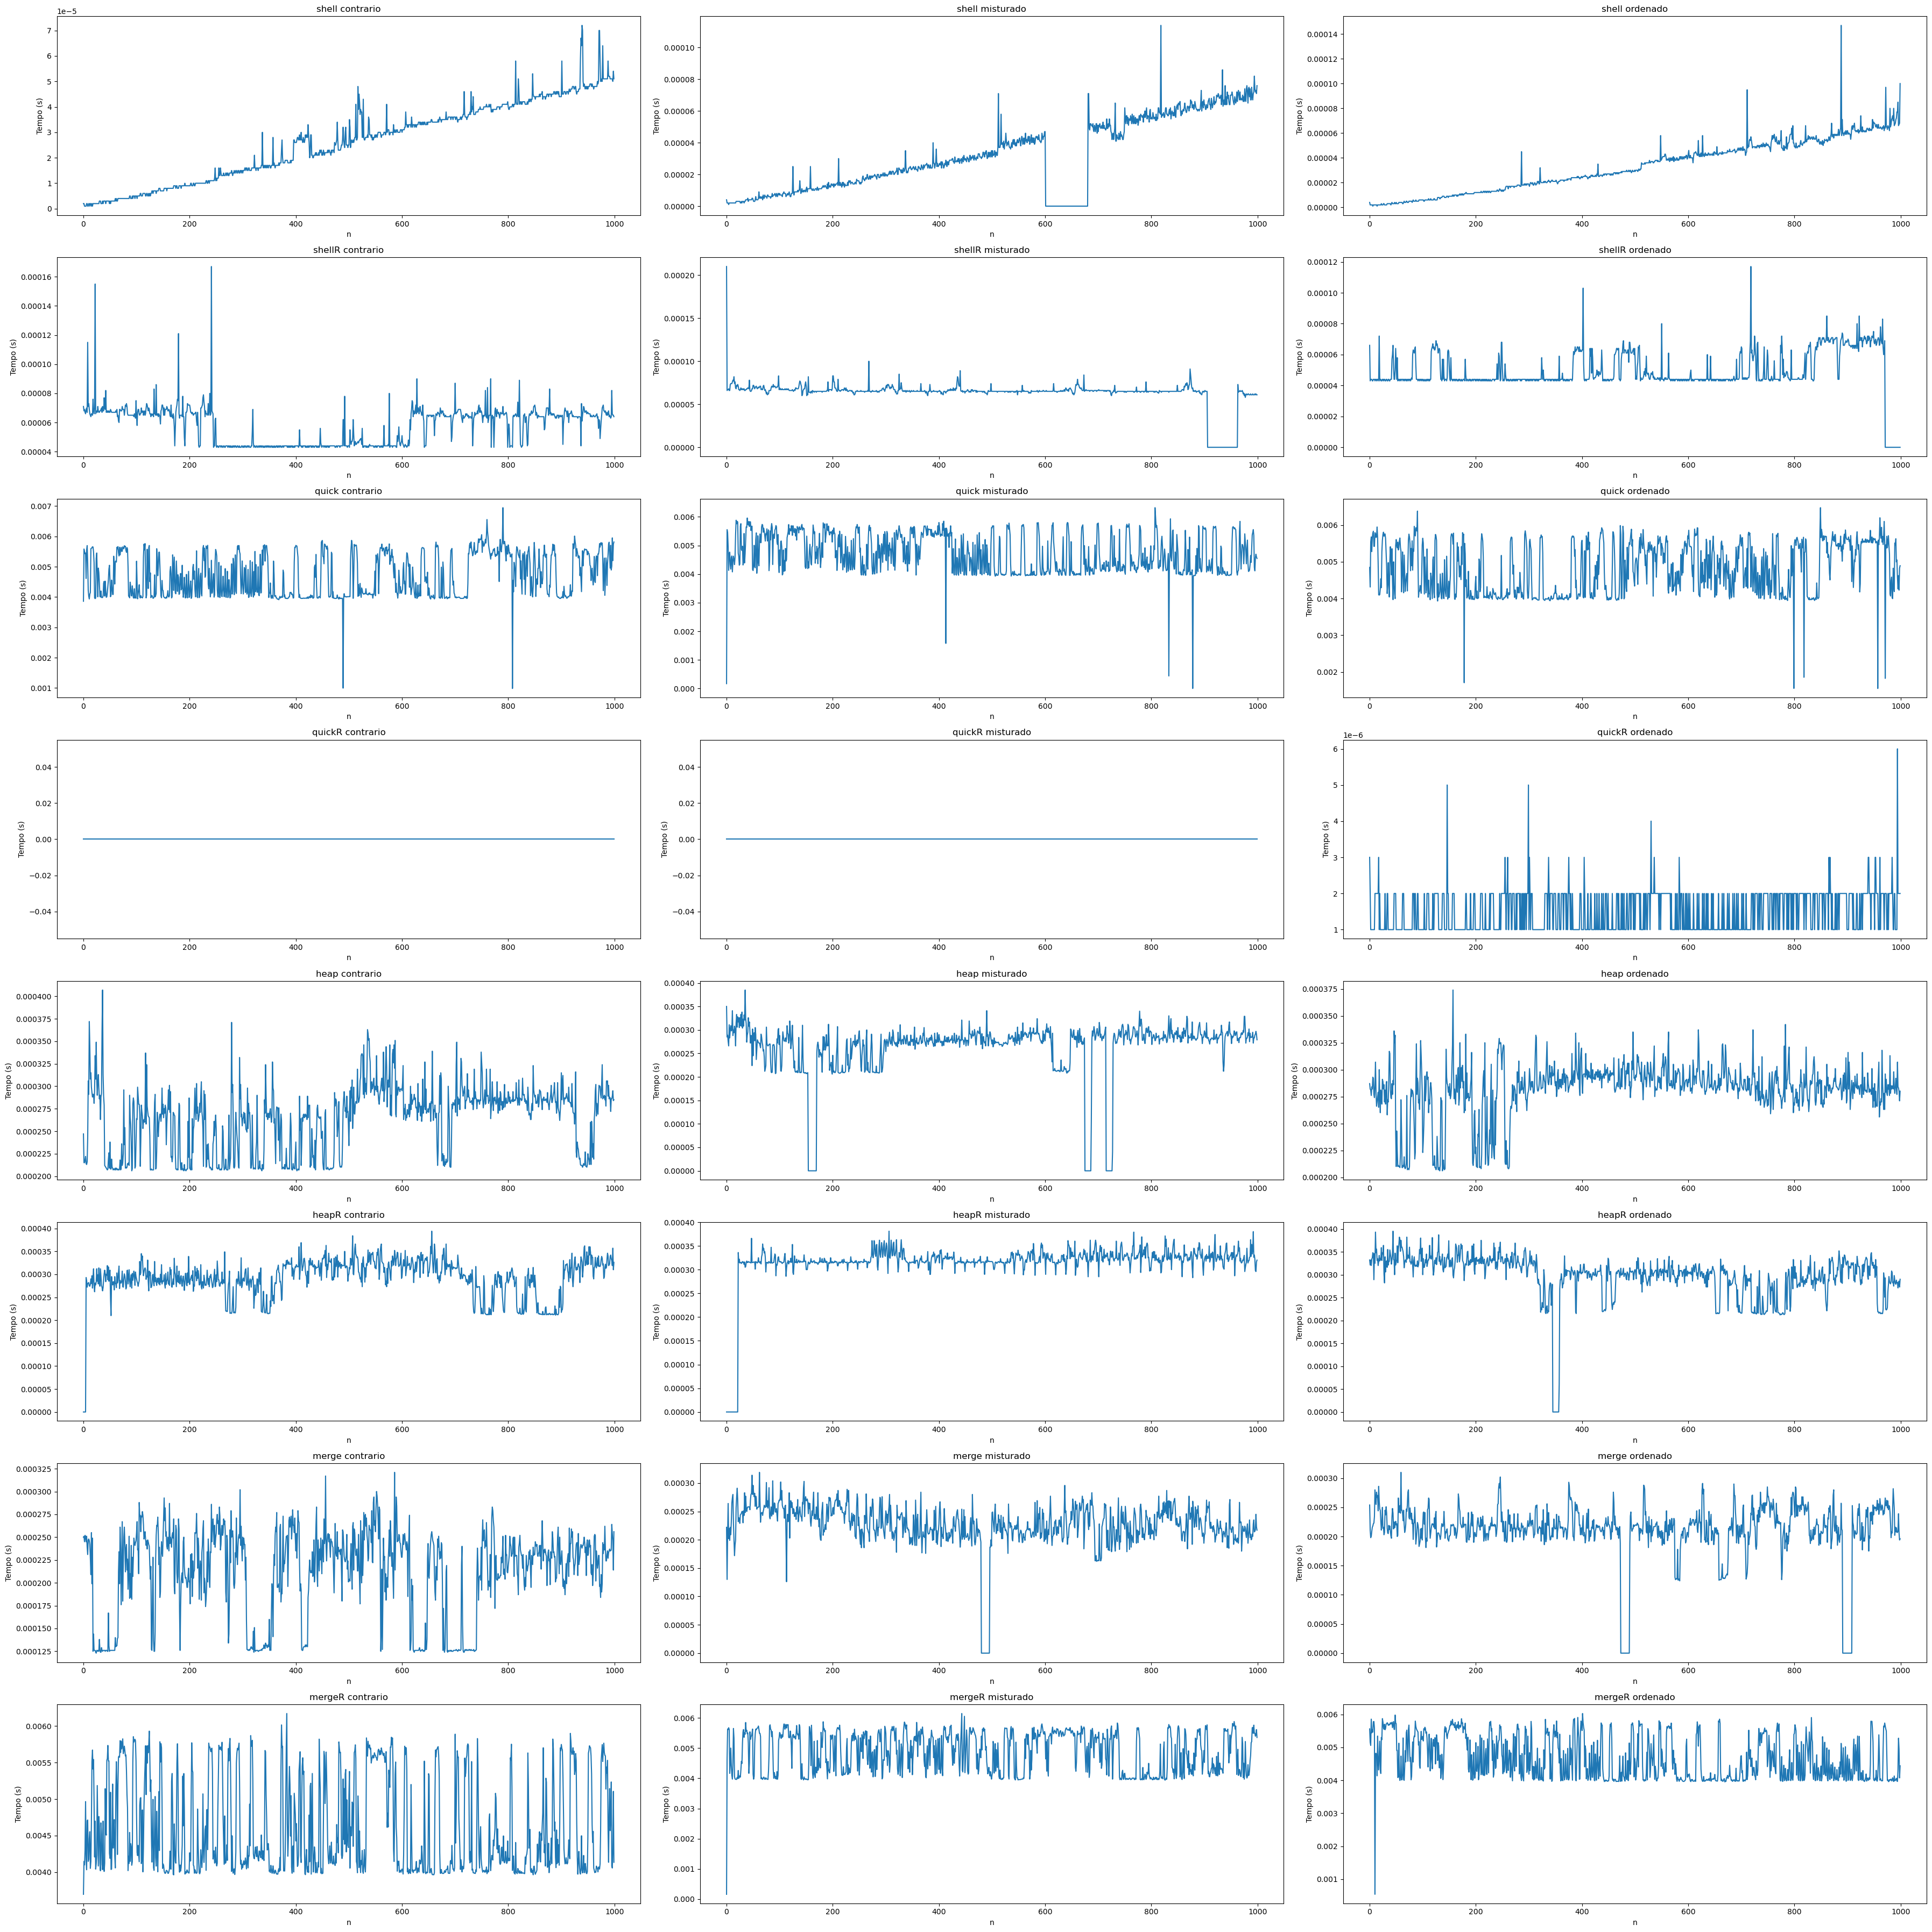
\includegraphics[width=1\linewidth]{imgs/tempo}
	\caption{Algoritmos vs tempo vs $n$}
	\label{fig:tempo}
\end{figure}

\section{Códigos}

\lstinputlisting{../ex11/ordenacao.c}



